	\section{Exercise 5: Floating Manipulation}

	Use the DexROV simulation for this exercise.

	\subsection{Adding mission phases}
	\question
	Let us now structure the mission in more than one phase. In the first phase,
	exploit the previous exercises, and implement a safe waypoint navigation. Move
	the vehicle to a location close to the current defined end-effector goal
	position, just slightly above it. Then, trigger a change of action and perform
	floating manipulation.

	Goal: introduce mission phases in the floating manipulation scenario. Observe
	the difference.
	\begin{parts}
		\part{Report the unified hierarchy of tasks used and their
		priorities. Which task is active in which phase/action?}

		\begin{solutionorbox}
			The unified hierarchy of tasks used is described in
			Table~\ref{table:tkip_swn_fm_dexrov}. 

			For the Safe Waypoint Navigation, only two tasks are
			active, i.e. Horizontal Attitude and Vehicle position.
			For the Floating Manipulation, four tasks are active,
			i.e. Horizontal Attitude, Joint limits, Dexterity and
			End-effector position.
		\end{solutionorbox}
		
		\begin{table}[htb] 
			\caption{Hierarchy of tasks for Safe Waypoint Navigation
			\& Floating Manipulation - DexROV}
			\label{table:tkip_swn_fm_dexrov}
			\begin{center}
				\footnotesize
				\begin{tabular}{ccccc}
					\toprule Task & Type &
					Safe Waypoint Navigation & Floating
					Manipulation\\
					\midrule 
					\hdashline Horizontal attitude & I & 1
									& 1\\ 
					\hdashline Joint limits & I && 2\\
					\hdashline Dexterity & I && 3\\
					\hdashline Vehicle position & I & 2 \\ 
					\hdashline End-effector position & E
									 &&4\\ 
					\bottomrule
				\end{tabular}%
			\end{center}%
		\end{table}%

		\part{What is the difference if, from the very beginning, you use
		the action of floating manipulation (i.e. just a single action)?}

		\begin{solutionorbox}
			If the mission starts from the Floating Manipulation,
			instead of the Safe Waypoint Navigation, then the arm
			moves during the translation from the initial position
			to the objective position. The arm movements influence
			the vehicle from the beginning, which means some safety
			tasks might not be fully satified, e.g. Horizontal
			Attitude.
		\end{solutionorbox}

	\end{parts}

	\subsection{Adding an optimization control objective}
	\question
	The goal is to try to optimize the joint positions, if possible, to keep the
	first four joints in a "preferred shape", represented by the following vector

	\begin{displaymath}
		\vec{q}_{\pas} = 
		\begin{bmatrix}
			-0.0031 & 1.2586 & 0.0128 & -1.2460 & 0 & 0 & 0
		\end{bmatrix}\T
	\end{displaymath}

	Goal: Add an optimization objective to keep the first four joints of the
	manipulator in the preferred shape. Observe the behaviour with and without the
	task
	\begin{parts}
		\part{Report the hierarchy of tasks used and their priorities in
		each action. At which priority level did you add the optimization task?}
		
		\begin{solutionorbox}
			The unified hierarchy of tasks used is described in
			Table~\ref{table:tkip_swn_fmv2_dexrov}. 
	
			The optimization task is added to the bottom priority
			level.
		\end{solutionorbox}
		
		\begin{table}[htb] 
			\caption{Hierarchy of tasks for Safe Waypoint Navigation
			\& Floating Manipulation v2 - DexROV}
			\label{table:tkip_swn_fmv2_dexrov}
			\begin{center}
				\footnotesize
				\begin{tabular}{ccccc}
					\toprule Task & Type &
					Safe Waypoint Navigation & Floating
					Manipulation v2\\
					\midrule 
					\hdashline  Horizontal attitude & I & 1
									& 1\\ 
					\hdashline Joint limits & I && 2\\
					\hdashline Dexterity & I && 3\\
					\hdashline Vehicle position & I & 2 \\ 
					\hdashline End-effector position & E
									 &&4\\ 
					\hdashline Preferred arm shape & I
									 &&5\\ 
					\bottomrule
				\end{tabular}%
			\end{center}%
		\end{table}%

		\part{What is the Jacobian relationship for the Joint Preferred
		Shape task? How was the task reference computed?}

		\begin{solutionorbox}
			The Jacobian $\J_{\pas}$ is identical to the Joint
			limits' Jacobian, i.e.
			\[
				\J_{\pas} = \begin{bmatrix}
					\Inm77\quad
					\Znm66
				\end{bmatrix}
				\mathrm{.}
			\]

			The desired references values correpond to the preferred
			arm shape, 

			\[
				 \xdotbar\pas = 
				\lambda\left(\vec{q}_{\pas} - \vec{q}\right)\quad
				\lambda\in\mathbb{R}^+
				\mathrm{,}
			\]	 			
		\end{solutionorbox}
		
		\part{What is the difference between having or not having this
		objective?}

		\begin{solutionorbox}
			Given the preferred arm shape, the difference shows not
			only in the final position and orientation of the
			vehicle, but also in the dexterity of the arm. Comparing
			the manipulability with and without the preferred arm
			shape optimization task, it is obvious that the task
			improves the manipulability of the arm over time, which
			reduces the risk of reaching a kinematic singularity.

			On Figure~\ref{fig:ex5_mu}, we can see that the
			manipulability measure reaches much lower values during
			the Floating Manipulation task around 30s without the
			optimization task. 

			Equally, the optimization task affects the paths chosen
			by the TPIK algorithm, leading the vehicle to move
			differently with the task active than without in order
			to keep the preferred arm shape.
		\end{solutionorbox}

		\begin{figure}[ht]
			\centering
			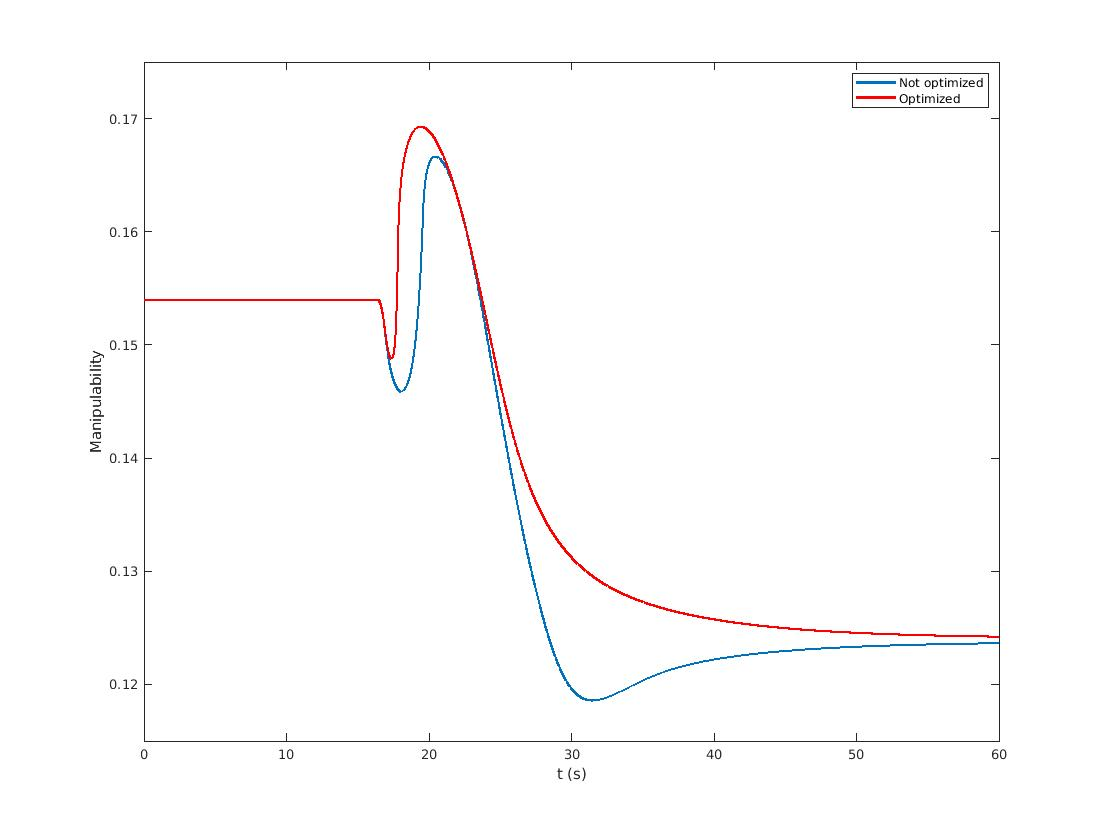
\includegraphics[width=0.6\linewidth]{manipulability.jpg}
			\caption{Manipulability measure with and without
				preferred arm shape task}%
			\label{fig:ex5_mu}
		\end{figure}
	\end{parts}
